\section{Algorithm}
\label{sec:alg}

Given a shape $\mathbb{S}$, our algorithm mainly performs the following three steps (as illustrated in Figure~\ref{fig:Eager}). 1) Automatically decompose the shape into some pieces. 2) For each piece $\mathbb{S}_i$, match the remaining shape $\mathbb{S}-\mathbb{S}_i$ to $\mathbb{S}_i$ such that for any node in  $\mathbb{S}-\mathbb{S}_i$, a partial match from $\mathbb{S}_i$ is performed. 3) Put together all the correspondences to form a many-to-many correspondence in $\mathbb{S}$, and cluster nodes in $\mathbb{S}$ based on local transformation consistency of the matching.

\begin{figure*}[t!]
\centering
  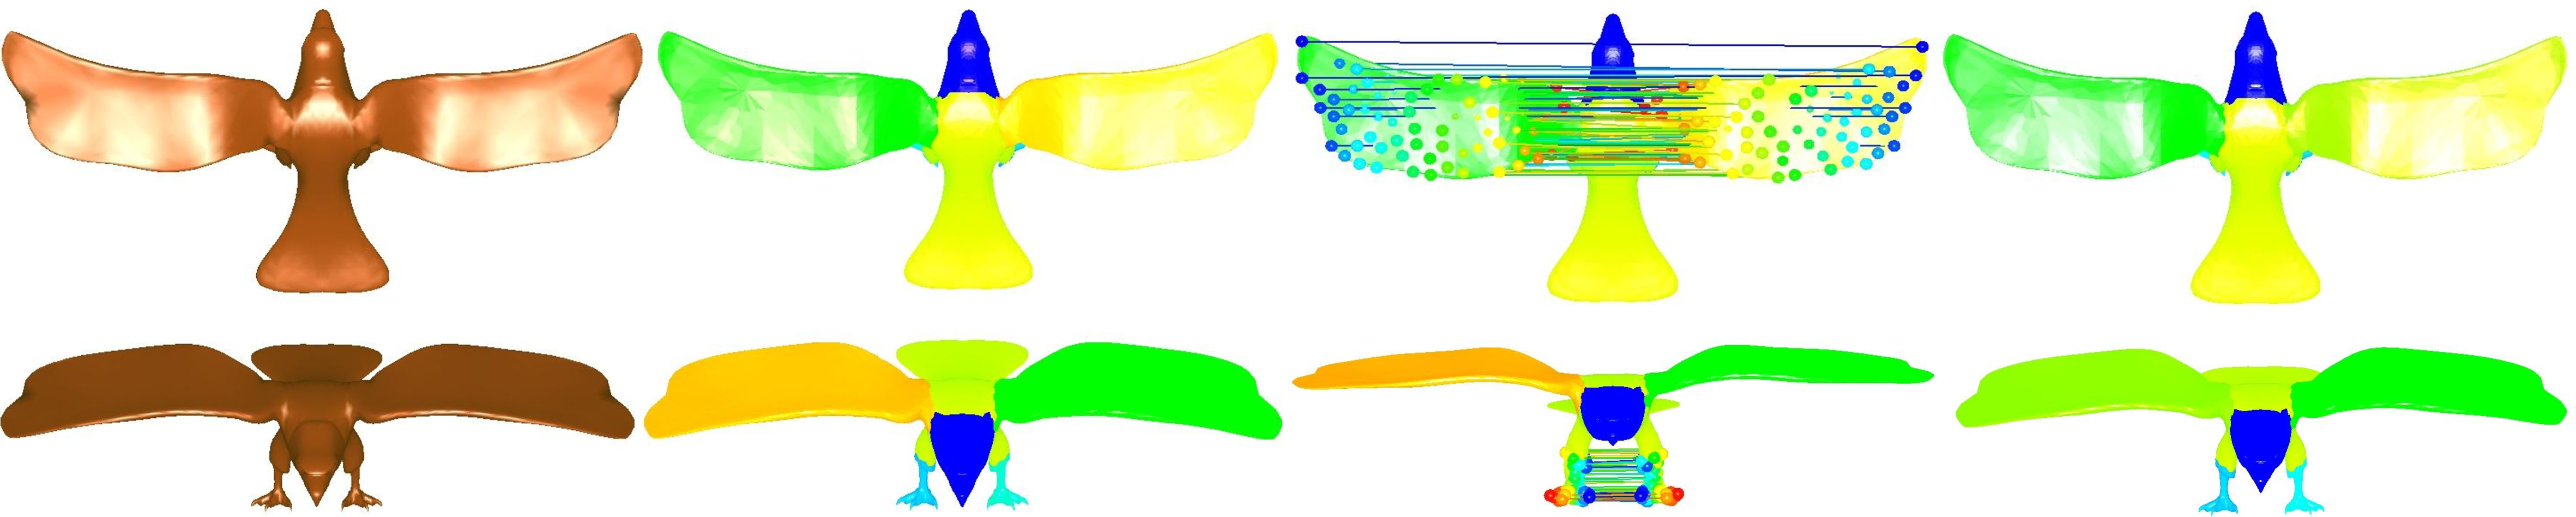
\includegraphics[width=0.99\linewidth]{figures/pipe.pdf}
  \caption{Algorithm pipeline (demonstrated by the Eager example from two viewpoints).
  From left to right, for a given shape, our algorithm decomposes it into several parts, matches each part to the remaining shape, then detect the symmetry by clusternig the correspondences based on the consistency of the matching. }
\label{fig:Eager}
\end{figure*}

\subsection{Automatic meaningful segmentation}
\label{subsec:segmentation}

For the input shape $\mathbb{S}$, in order to find the generalized intrinsic partial symmetry, we decompose the model into $n$ pieces: $\mathbb{S}_1$, $\mathbb{S}_2$, $\dots$, $\mathbb{S}_n$.
The segmentation should ideally lead to each region representing a meaningful part of the object. We used random walks based segmentation~\cite{lai2009} which involves distributing $n$ seeds as far away as possible over the surface and segmenting the shape by assigning a label to each face/point, indicating the seed with the maximum probability to be hit by a random walker starting from the face. The probability of movement is derived from the local geometry such that it is more difficult to move across sharp edges. Implied by the existing symmetry detection algorithms~\cite{xu2009,berner2011}, symmetric parts are always meaningful. This is the foundation of our algorithm and could explain why the meaningful segmentation is first performed to provide the parts for symmetry detection, although the other surface-based segmentation algorithm could also provide the initial segmentation.

\subsection{Partial matching}
\label{subsec:matching}

In order to find the symmetries, we uniformly sample the shape $\mathbb{S}$ with $m$ samples,
and then build the partial matching between every pair of regions $\mathbb{S}_i$ and $\mathbb{S}_j$, $i \neq j$.

The partial matching is achieved by a third-order tensor matching algorithm [reference omitted for review],
which is improved from the tensor-based algorithm for high-order graph matching~\cite{Duchenne2011}.
Our algorithm formulates the matching using a supersymmetric tensor representing an affinity metric,
which takes into account feature similarity and geometric constraints between features.
Note that, although~\cite{Duchenne2011} claimed to use a supersymmetric affinity tensor,
their approach did not make full use of supersymmetry when creating the supersymmetric affinity tensor, nor does it take advantage of supersymmetry
to accelerate the power iteration process and sampling.
Going beyond~\cite{Duchenne2011}, our algorithm [reference omitted for review] really takes advantage of supersymmetry to devise an
efficient sampling strategy to estimate the affinity tensor, as well as to store the estimated tensor compactly.
Matching is performed by an efficient higher-order power iteration approach which takes advantage of the compact representation of the supersymmetric affinity tensor.
efficient sampling strategy to estimate the affinity tensor, as well as to store the estimated tensor compactly.

The algorithm matches samples using a pair of three-tuples from both shapes and ensures consistency in geodesic distances.
To speed up the geodesic distance computation, the approximate Dijkstra algorithm~\cite{Dijkstra1959} is adopted and performed on the sampled points.
Assume the number of matches between regions $\mathbb{S}_i$ and $\mathbb{S}_j$ is $match_{i,j}$,
the regions are recognized as of candidate symmetry if $match_{i,j} > cm$, where $c$ is a constant and typically assigned as $0.2/n$ and $m$ equals to $100 \times n$
for all examples in the paper.


\subsection{Correspondences clustering}

In the following, we put together all the correspondences for each part $\mathbb{S}_i$, found by former partial matching.
So, we form a many-to-many correspondence in the whole $\mathbb{S}$.
Then, we cluster nodes in $\mathbb{S}$ based on local transformation consistency of the matching.

Benefiting from our partial matching, rigid transforms can be computed from each triple of compatible matching points.
The transform which brings the most data points within a threshold distance of a point in the model is chosen as the optimal alignment transform~\cite{Huttenlocher1990}.
As shown by ~\cite{Huttenlocher1990}, this transformation always exists for three non-collinear points, and is unique up to a reflective ambiguity.
The solution method is closed-form and only involves second-order equations.
The later paper~\cite{Gelfand05} claimed that such a voting scheme is robust to the initial pose of the triples.

Our clustering method is similar to~\cite{mitra2006} based on the computed transformation that map local surface patches onto each other.
Each matching pair provides evidence for a symmetry relation at the level of the local sample spacing.
So, we could extract meaningful symmetries at larger scales by finding groups of pairs with a similar transformation
that correspond to symmetric subsets of the shape.
The suitable clustering method also is mean shift clustering~\cite{Comaniciu2002}, a non-parametric method based on gradient ascent on a density function.










